\documentclass[varwidth,border={1cm 0.5cm 1cm 0.5cm}]{standalone} %E,S,W,N

\usepackage{amssymb}
\usepackage{amsmath}	%for labels
\usepackage{tikz}

%spectral analysis of economic time series -- Fig. 1: Signal and its decomposition
%Cooper, R. (1972). ``The Use of Spectral Analytic Techniques in Economics.'' RAND Research Paper P-4882. Santa Monica: RAND Corporation, p. 5 Retrieved from www.rand.org/pubs/papers/P4882.html

\begin{document}
	
	\hspace{-1cm}%			%have to play with margins because {standalone}
	\begin{tikzpicture}
	%AXIS
	\draw (0,0)--(13,0);			%horizontal axis
	\draw (0,-3)--(0,3);			%vertical axis
	\foreach \x in {-3,...,3}{		%vertical numbers
		\draw (0,\x)--(0.15,\x);	%vertical ticks
		\node[align=right,left] at (0,\x) {\small $\x$};
	}
	\foreach \x in {0,...,13} \draw (\x,-0.1)--(\x,0.1); %horizontal ticks, middle
	\node at (0,3.6)   {\small $x(t)$};
	\node at (13,0.4)  {\small $t$};
	\node at (6.5,2.5) {(a) Continuous signal $x(t)$};
	
	%PLOT
	\draw[thick,domain=0:13,samples=100] 
	plot (\x,{2*cos(0.625/1.2*\x r) + sin(1.25/1.2*\x r) + 0.5*cos(2.5/1.2*\x r)});
	
%	\draw[help lines] (0,-4) grid (13,4);
	\end{tikzpicture}
	
	
	\vspace{0.5cm}
	
	\hspace{-1cm}%
	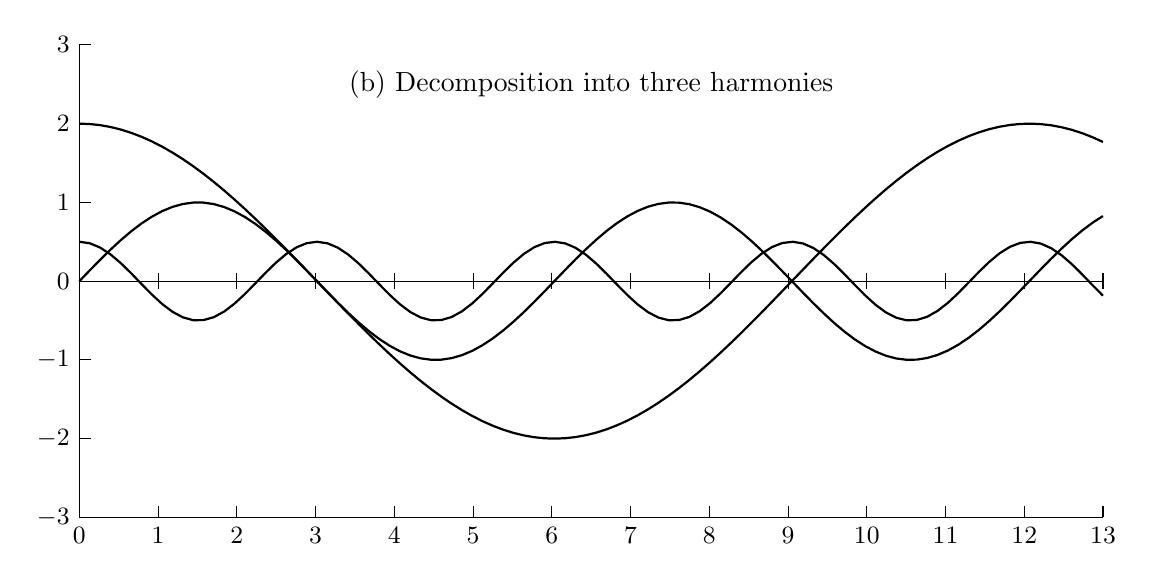
\begin{tikzpicture}
	%AXIS
	\draw (0,0)--(13,0);				%horizontal, middle
	\draw (0,-3)--(13,-3);				%horizontal, bottom
	\draw (0,-3)--(0,3);				%vertical
	\foreach \x in {-3,...,3}{ 			%vertical numbers
		\draw (0,\x)--(0.15,\x);		%vertical ticks
		\node[align=right,left] at (0,\x) {\small $\x$};
	}
	\foreach \x in {0,...,13}{			%horizontal numbers
		\draw (\x,-0.1)--(\x,0.1);		%horizontal ticks, middle
		\draw (\x,-3)--(\x,-2.85);		%horizontal ticks, bottom
		\node[align=center,below] at (\x,-3) {\small $\x$};
	}
	\node at (6.5,2.5) {(b) Decomposition into three harmonies};
	
	%PLOT
	\draw[thick,domain=0:13,samples=100] plot (\x,{2*cos(0.625/1.2*\x r)});	%big cosine
	\draw[thick,domain=0:13,samples=100] plot (\x,{sin(1.25/1.2*\x r)});	%medium sine
	\draw[thick,domain=0:13,samples=100] plot (\x,{0.5*cos(2.5/1.2*\x r)});	%small cosine
	
%	\draw[thick,domain=0:10.83] plot (1.2*\x,{2*cos(0.625*\x r)});	%big cosine
%	\draw[thick,domain=0:21.67] plot (0.6*\x,{sin(0.625*\x r)});	%medium sine
	
%	\draw[help lines] (0,-3) grid (13,3);
	\end{tikzpicture}
	
\end{document}